\chapter{Desarrollo}
\label{ch:desarrollo}

Este capítulo detalla el desarrollo técnico del trabajo, incluyendo el diseño, la implementación y los aspectos más relevantes del proceso.

\section{Análisis de requisitos}

\subsection{Requisitos funcionales}

\begin{itemize}
  \item \textbf{RF01:} El sistema debe permitir...
  \item \textbf{RF02:} El usuario podrá...
  \item \textbf{RF03:} Se implementará...
\end{itemize}

\subsection{Requisitos no funcionales}

\begin{itemize}
  \item \textbf{RNF01:} El tiempo de respuesta no debe superar los 2 segundos.
  \item \textbf{RNF02:} El sistema debe soportar al menos 100 usuarios concurrentes.
  \item \textbf{RNF03:} La interfaz debe ser accesible según WCAG 2.1.
\end{itemize}

\section{Diseño del sistema}

\subsection{Arquitectura general}

La arquitectura del sistema sigue un patrón de capas, como se muestra en la Figura~\ref{fig:arquitectura}.

\begin{figure}[htbp]
  \centering
  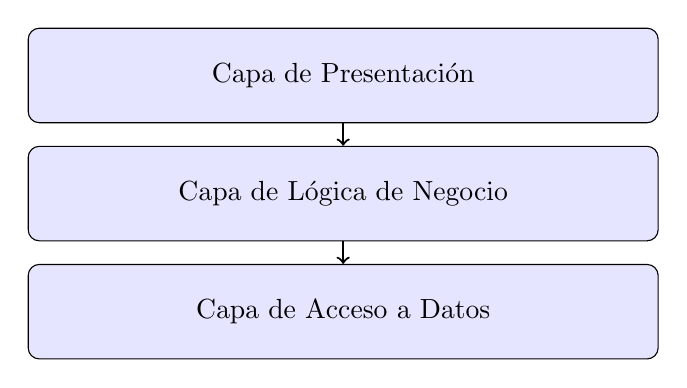
\begin{tikzpicture}[
    capa/.style={draw, rounded corners, minimum width=8cm, minimum height=1.2cm, fill=blue!10},
    flecha/.style={->, thick}
  ]
    \node[capa] (presentacion) at (0,3) {Capa de Presentación};
    \node[capa] (logica) at (0,1.5) {Capa de Lógica de Negocio};
    \node[capa] (datos) at (0,0) {Capa de Acceso a Datos};
    
    \draw[flecha] (presentacion) -- (logica);
    \draw[flecha] (logica) -- (datos);
  \end{tikzpicture}
  \caption{Arquitectura en capas del sistema}
  \label{fig:arquitectura}
\end{figure}

\section{Implementación}

\subsection{Estructura del proyecto}

El proyecto está organizado de la siguiente manera:

\begin{bashcode}
proyecto/
├── src/
│   ├── main.py
│   ├── models/
│   └── utils/
├── tests/
├── docs/
└── requirements.txt
\end{bashcode}

\subsection{Ejemplo de código Python}

A continuación se muestra un ejemplo de implementación en Python:

\begin{pythoncode}[title={Clase principal del sistema}]
class SistemaGestion:
    """Clase principal para la gestión del sistema."""
    
    def __init__(self, config: dict):
        self.config = config
        self.conexion = None
    
    def conectar(self) -> bool:
        """Establece la conexión con la base de datos."""
        try:
            self.conexion = BaseDatos(self.config['db'])
            return True
        except Exception as e:
            print(f"Error de conexión: {e}")
            return False
    
    def procesar_datos(self, datos: list) -> dict:
        """Procesa los datos recibidos."""
        resultados = {}
        for item in datos:
            resultados[item['id']] = self._calcular(item)
        return resultados
\end{pythoncode}

\subsection{Ejemplo de código JavaScript}

Para el frontend se ha utilizado JavaScript moderno:

\begin{jscode}[title={Componente de interfaz}]
async function cargarDatos(endpoint) {
    try {
        const response = await fetch(endpoint);
        const data = await response.json();
        
        return data.map(item => ({
            id: item.id,
            nombre: item.nombre,
            fecha: new Date(item.fecha)
        }));
    } catch (error) {
        console.error('Error al cargar datos:', error);
        throw error;
    }
}
\end{jscode}

\subsection{Consultas SQL}

La base de datos utiliza las siguientes consultas principales:

\begin{sqlcode}[title={Consulta de usuarios activos}]
SELECT 
    u.id,
    u.nombre,
    u.email,
    COUNT(s.id) AS total_sesiones
FROM usuarios u
LEFT JOIN sesiones s ON u.id = s.usuario_id
WHERE u.activo = TRUE
    AND s.fecha > CURRENT_DATE - INTERVAL '30 days'
GROUP BY u.id, u.nombre, u.email
ORDER BY total_sesiones DESC
LIMIT 100;
\end{sqlcode}

\section{Pruebas realizadas}

\subsection{Pruebas unitarias}

Se han implementado pruebas unitarias para todos los componentes críticos del sistema:

\begin{pythoncode}[title={Ejemplo de test unitario}]
import pytest
from sistema import SistemaGestion

class TestSistemaGestion:
    def test_conexion_exitosa(self, config_test):
        sistema = SistemaGestion(config_test)
        assert sistema.conectar() == True
    
    def test_procesar_datos_vacio(self):
        sistema = SistemaGestion({})
        resultado = sistema.procesar_datos([])
        assert resultado == {}
\end{pythoncode}
